\documentclass[../p164main.tex]{subfiles}
\graphicspath{{\subfix{../figures/}}}

\usepackage{mhchem}
\ExplSyntaxOn
\keys_define:nn { mhchem }
 {
  arrow-min-length .code:n =
   \cs_set:Npn \__mhchem_arrow_options_minLength:n { {#1} } % default is 2em
 }
\ExplSyntaxOff
\mhchemoptions{arrow-min-length=1em}

\usepackage[compat=1.1.0]{tikz-feynman}
\tikzset{rubout/.style={preaction={draw=white,line width=3pt}}}     % makes crossing lines less confusing

\begin{document}

\chapter{Unsorted Notes}
% \section{Overview (Lecture 1)}
% Particle physics is the study of the elementary constituents of matter---that is, of the minimal subset of matter that can explain all the phenomena we see.
% Our current understanding of these particles is formalized by the Standard Model (SM), which consists of a whole bunch of distinct particles and three forces describing the interactions between them.

% \medskip

% \begin{center}
%     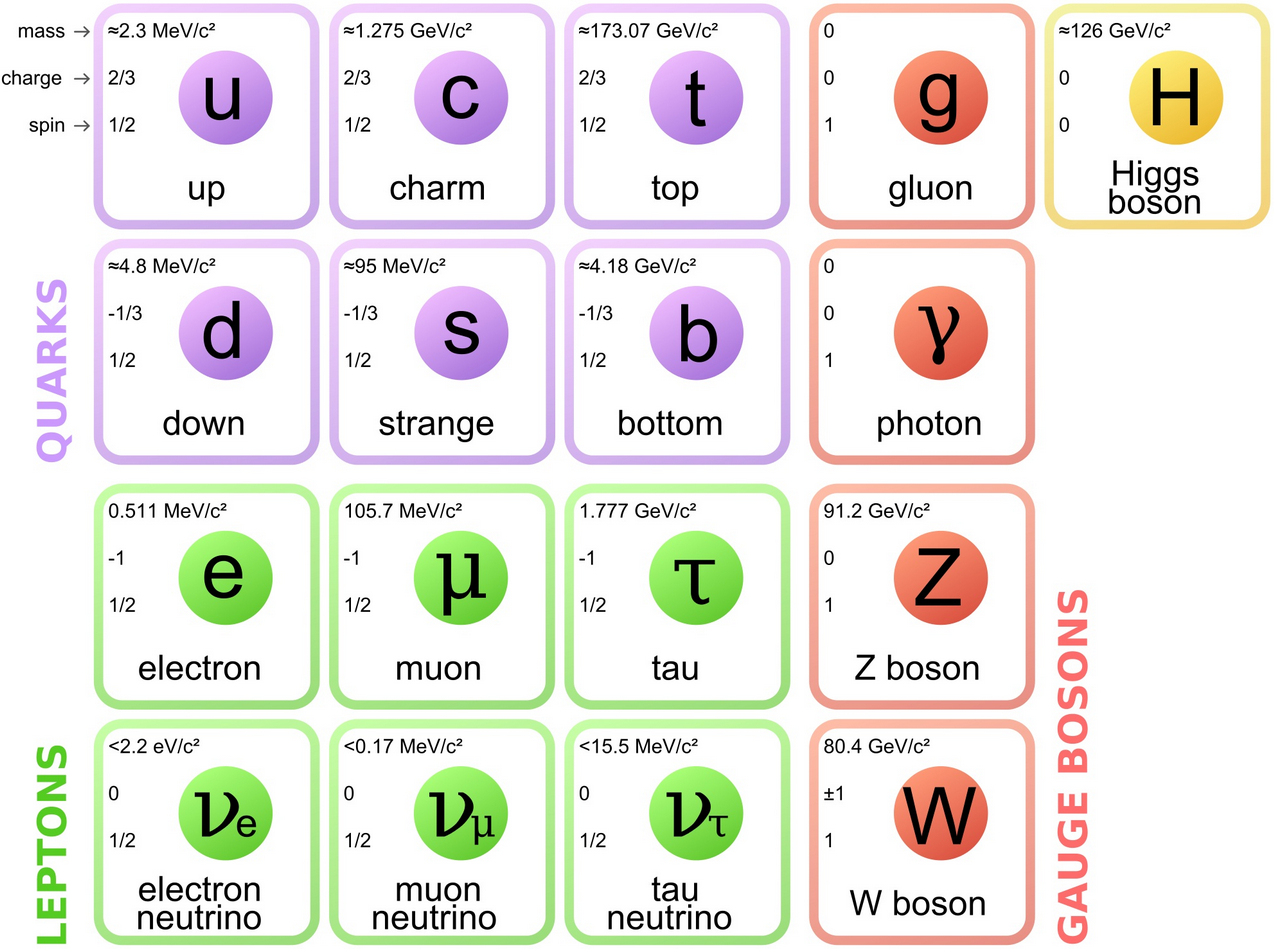
\includegraphics[width=0.75\textwidth]{standardModel.png}
% \end{center}

% Each particle here has a corresponding antiparticle of opposite charge.
% For example, $e^- \leftrightarrow e^+$, $p^+ \leftrightarrow \overline p^-$, and $\gamma \leftrightarrow \gamma$.
% (Note that neutral particles are not necessarily their own antiparticle!)
% The gauge bosons mediate force interactions between particles, and the Higgs boson is what gives particles their mass.

% A particle's charge determines how it interacts with the electromagnetic force, so some particles feel it and others don't.
% Particles may or may not also interact with the strong force---quarks do, and leptons don't.
% All particles interact with the weak force, though the nature of this interaction is complicated.

% The behavior of each force depends on two properties: the mass of the force carrier, and some dimensionless coupling strength $\alpha$.
% The electromagnetic force, for example, is mediated by the massless photon $\gamma$.
% We can write the electrostatic potential between two electrons as
% \[ U(\mbf{r}) = \hbar c \left( \frac{\alpha_\textrm{EM}}{r} \right), \qquad \alpha_\textrm{EM} = \frac{q_e^2}{4\pi \epsilon_0 \hbar c} \approx \frac{1}{137}, \]
% where $\alpha_\textrm{EM}$ is the coupling strength for electromagnetism.
% As we'll see, the probability of a scattering event occurring is proportional to $\alpha_\textrm{EM}^2$.

% The weak force has coupling strength $\alpha_W = 0.032$.
% This is very clearly larger than $\alpha_\text{EM}$, which suggests that the weak force is actually stronger than the electromagnetic force.
% We resolve this apparent misnomer by noting that the mediators of the weak force---the $W^\pm$ and $Z$ bosons---are very heavy, much heavier than even a proton.
% We thus modify the potential to get the Yukawa potential
% \[ U(r) = -\hbar c \left( \frac{\alpha_W}{r} \right) e^{-r / R_W}, \qquad R_W = \frac{\hbar}{cm_Z}. \]
% So heavy mediators give rise to short-range forces.
% For particles with very large de Broglie wavelengths compared to $R_W$ the potential looks more like
% \[ U(\mbf{r}) = -4\pi \alpha_W R_W^2 \,\delta^3(\mbf{r}), \]
% and in this case the coupling is modified to $4\pi \alpha_W R_W^2$.
% To get a dimensionless scattering probability we introduce the wavenumber $k$ to get $P \sim (\pi \alpha_W k^2 R_W^2)^2$, and since $p \approx E / c$ for a relativistic particle, we find
% \[ P \sim \left( 4\pi \alpha_W \frac{E^2}{m_W^2 c^{4}} \right)^2. \]
% We can see that the weak force is ``weak'' at everyday energies, which are much lower than $m_W c^2$ and $m_Z c^2$.
% But at high energies the weak force is actually stronger than electromagnetism!

% The strong force, mediated by the gluon, has ``color charges'' red, green, and blue (along with their corresponding anti-colors).
% Its coupling strength is $\alpha_S \approx 0.1$, which isn't that much larger than $\alpha_W$.
% The reason we call it the strong force, then, has to do with the fact that the coupling $\alpha$ is not actually constant!

% $\alpha_\textrm{EM}$, for example, increases with increasing energy.
% (This has to do with vacuum polarization---when a charged particle and antiparticle spontaneously come into existence they create a dipole moment for a very small amount of time, which may be oriented depending on how close it is to a nearby charge.)
% The strong force, in contrast, gets weaker at higher energies as quarks and gluons get bound up into color-neutral hadrons.
% This ``binds up'' the strong force into larger particles (baryons), so we don't see its effects in everyday life.

% \section{Feynman Diagrams (Lecture 2)}
% Suppose we observe an electron and positron with momenta $\mbf{p}_1, \mbf{p}_2$ turn into a muon and antimuon with $\mbf{p}_3, \mbf{p}_4$; the amplitude of this occurring is denoted by $\braket{\mu^-(\mbf{p}_3), \mu^+(\mbf{p}_4)}{e^-(\mbf{p}_1), e^+(\mbf{p}_4)}$.
% But we can only observe the initial and final state of these particles---in principle, a whole variety of things could've happened in between!
% We can represent this by inserting the identity operator between the bra and ket:
% \[ \braket{\mu^-(\mbf{p}_3), \mu^+(\mbf{p}_4)}{e^-(\mbf{p}_1), e^+(\mbf{p}_4)} = \sum_{X}^{} \braket{\mu^-(\mbf{p}_3), \mu^+(\mbf{p}_4)}{X} \braket{X}{e^-(\mbf{p}_1), e^+(\mbf{p}_4)}. \]
% We describe the intermediate stages using Feynman diagrams.
% Each vertex of such a diagram represents an interaction with a force mediator, and at each vertex a number of quantities is conserved:
% \begin{itemize}[topsep=0pt]
%     \item energy and momentum,
%     \item electric charge and color charge,
%     \item quark number ($N_q, N_{\overline q}$) and baryon number $B = \frac{1}{3} (N_q - N_{\overline q})$, and
%     \item lepton number, including electron number, muon number, and tau number:
%     \begin{align*}
%         L_e &= (N_e + N_{\nu_e}) - (N_{\overline e} + N_{\overline{\nu}_e}), \\
%         L_\mu &= (N_\mu + N_{\nu_\mu}) - (N_{\overline \mu} + N_{\overline{\nu}_\mu}), \\
%         L_\tau &= (N_\tau + N_{\nu_\tau}) - (N_{\overline \tau} + N_{\overline{\nu}_\tau}).
%     \end{align*}
% \end{itemize}
% We'll start simple with the electromagnetic vertex, drawn below.
% (We could've put any charged particle-antiparticle pair here, we just use electrons for simplicity.)
% Time flows in the rightward direction, so we can orient the vertex in a number of ways to get different processes, being careful to conserve charge.
% \begin{center}
%     \feynmandiagram[small, horizontal = i1 to c]{
%         i1[particle = $\gamma$] --[photon] c,
%         c --[fermion] f1[particle = $e^-$],
%         c --[anti fermion] f2[particle = $e^+$]
%     }; \qquad
%     \feynmandiagram[small, horizontal = c to f1]{
%         i2[particle = $e^-$] --[fermion] c,
%         i1[particle = $e^+$] --[anti fermion] c,
%         c --[photon] f1[particle = $\gamma$]
%     }; \qquad
%     \feynmandiagram[small]{
%         i1[particle = $\gamma$] --[photon] c,
%         c --[fermion] f1[particle = $e^-$],
%         c --[anti fermion] f2[particle = $e^-$]
%     }; \qquad
%     \feynmandiagram[small]{
%         i1[particle = $\gamma$] --[photon] c,
%         c --[fermion] f1[particle = $e^+$],
%         c --[anti fermion] f2[particle = $e^+$]
%     };
% \end{center}
% Each of these vertices corresponds to an amplitude $\sim \sqrt{\alpha_\textrm{EM}}$.
% (This factor depends on the charge of the particles---up quarks, for example, have amplitude $\sim (2 / 3) \sqrt{\alpha_\textrm{EM}}$.)
% We can combine them to create more complex processes, like electron-electron scattering.
% \begin{center}
%     \feynmandiagram[small, vertical = c11 to c12, remember picture]{
%         i1[particle = $e^-(\mbf{p}_1)$] --[fermion] c11,
%         i2[particle = $e^-(\mbf{p}_2)$] --[opacity=0] c12,
%         c11 --[opacity=0] c12,
%         c21 --[opacity=0] c22,
%         c11 --[opacity=0] c21,
%         c12 --[opacity=0] c22,
%         c22 --[fermion] f2[particle = $e^-(\mbf{p}_4)$],
%         c21 --[opacity=0] f1[particle = $e^-(\mbf{p}_3)$],
%     }; \begin{tikzpicture}[overlay, remember picture]
%     \begin{feynman}
%         \path (c11) -- (f1)
%               (i2) -- (c22)
%               (c11) -- (c22);
%         \diagram*{
%             (c11) --[fermion] (f1),
%             (i2) --[fermion] (c22),
%             (c11) --[photon] (c22)
%         };
%     \end{feynman}
%     \end{tikzpicture}
%     \qquad
%     \feynmandiagram[small, vertical = c11 to c12, remember picture]{
%         i1[particle = $e^-(\mbf{p}_1)$] --[opacity=0] c11,
%         i2[particle = $e^-(\mbf{p}_2)$] --[fermion] c12,
%         c11 --[opacity=0] c12,
%         c21 --[opacity=0] c22,
%         c11 --[opacity=0] c21,
%         c12 --[opacity=0] c22,
%         c22 --[opacity=0] f2[particle = $e^-(\mbf{p}_4)$],
%         c21 --[fermion] f1[particle = $e^-(\mbf{p}_3)$],
%     }; \begin{tikzpicture}[overlay, remember picture]
%     \begin{feynman}
%         \path (c12) -- (f2)
%               (i1) -- (c21)
%               (c12) -- (c21);
%         \diagram*{
%             (c12) --[fermion] (f2),
%             (i1) --[fermion] (c21),
%             (c12) --[photon] (c21)
%         };
%     \end{feynman}
%     \end{tikzpicture}
% \end{center}
% The particles in the interior of a Feynman diagram are called virtual particles---they can't be directly observed, but they're useful fictions for doing calculations.
% This means, however, that we cannot distinguish between the above two processes, so we can ``sum'' them up in the following shorthand (on the left).
% \begin{center}
%     \feynmandiagram[small, vertical = c1 to c2]{
%         i1[particle = $e^-(\mbf{p}_1)$] --[fermion] c1,
%         i2[particle = $e^-(\mbf{p}_2)$] --[fermion] c2,
%         c1 --[photon] c2,
%         c1 --[fermion] f1[particle = $e^-(\mbf{p}_3)$],
%         c2 --[fermion] f2[particle = $e^-(\mbf{p}_4)$]
%     }; \qquad
%     \feynmandiagram[small, horizontal = i2 to f2, remember picture]{
%     i1[particle = $e^-(\mbf{p}_1)$] --[fermion] c1,
%     i2[particle = $e^-(\mbf{p}_2)$] --[fermion] c2,
%     c1 --[photon] c2,
%     c1 --[ghost,opacity=0] f1[particle = $e^-(\mbf{p}_3)$],  % phantom edge to keep p_3 in place
%     c2 --[ghost,opacity=0] f2[particle = $e^-(\mbf{p}_4)$]   % "                  " p_4 in place
%     }; \begin{tikzpicture}[overlay, remember picture]
%     \begin{feynman}
%     \path (c1) -- (f2) coordinate[midway] (p1)  % creates a point midway between c1 and f2
%           (c2) -- (f1) coordinate[midway] (p2); % "                            " c2 and f1
%     \diagram*{
%     (c1) -- (p1) -- [fermion] (f2),             % cuts c1 -> f2 into two segments for arrow clarity
%     (c2) --[rubout] (p2) -- [fermion] (f1)      % cuts c2 -> f1 "                                 "
%     };
%     \end{feynman}
%     \end{tikzpicture}
% \end{center}
% Even with this shorthand, however, the scattering can still occur in two different (albeit indistinguishable) ways; the other one is above, on the right.
% So when we go to determine the probability of electron scattering occurring, we really have four distinct diagrams to consider.

% These four diagrams are what we call the leading-order diagrams for electron scattering.
% In principle there are infinitely many processes that have the same inputs and outputs, but all of them have more vertices, each contributing an extra $\sqrt{\alpha_\textrm{EM}}$ factor.
% If this factor is small, higher-order diagrams give subdominant contributions to the overall amplitude.

% Most strong-forces vertices look very similar: a gluon is attached to two quarks of the same type.
% One notable difference here is that gluons, unlike photons, are able to interact with one another in two different ways!
% So we get the following diagrams.
% (Here, $q$ denotes an arbitrary quark.)
% \begin{center}
%     \feynmandiagram[small, horizontal = i1 to c]{
%         i1[particle = $g$] --[gluon] c,
%         c --[fermion] f1[particle = $q$],
%         c --[anti fermion] f2[particle = $\overline q$]
%     }; \qquad
%     \feynmandiagram[small, horizontal = i1 to c]{
%         i1[particle = $g$] --[gluon] c,
%         c --[gluon] f1[particle = $g$],
%         c --[gluon] f2[particle = $g$]
%     }; \qquad
%     \feynmandiagram[small, horizontal = i1 to f1]{
%         i1[particle = $g$] --[gluon] c,
%         i2[particle = $g$] --[gluon] c,
%         c --[gluon] f1[particle = $g$],
%         c --[gluon] f2[particle = $g$]
%     };
% \end{center}
% The first two vertices have amplitude $\sqrt{\alpha_S}$, while the third has $\alpha_S$.
% Note that quarks can change color during interactions, meaning the gluon must carry away the difference.
% (Thus gluons are ``bi''-colored, with one unit of positive and another unit of negative color.)

% The fact that strong vertices are so similar to electromagnetic ones suggests that we can use different forces to get the same observed process.
% We technically have to sum all of the possible Feynman diagrams, but the diagrams associated with the stronger force are dominant.
% (For example, in the scattering of two up quarks the strong force dominates.)

% As a quick note, in practice it's common to do calculations in terms of the coupling constant
% \[ g = \sqrt{4\pi \alpha} \]
% in order to avoid all the square roots flying around.
% The electromagnetic coupling constant is denoted $g_e$ (or, annoyingly, $e$).
% This $g$, not $\alpha$, is the parameter that shows up in modern field theory.

% Now let's talk about the weak force.
% The vertices corresponding to the $Z$ boson are very similar to the previous ones, as it is coupled to a fermion and itself, or its antiparticle.
% (We call this coupling generation-diagonal.
% That is, there is no cross-generational coupling.)

% The $W$ bosons are a bit different, as its coupling occurs with two \textit{different} fermions.
% Further, its coupling to the leptons is generation-diagonal, but its coupling to the quarks is not!
% Any quark-quark pair can be coupled with a $W$ boson, so long as charge is conserved.
% Each vertex has a coupling constant that looks like $g_W V_{ud}$, in the case of up-down coupling.
% These are the only SM interactions that change generation (and quark flavor)!

% The key idea here is that there are two ways of defining down-type quarks.
% We may use the mass basis, in which $\ket{d}$, $\ket{s}$, and $\ket{b}$ are energy eigenstates; or we may use the interaction basis, in which $\ket{d'}$, $\ket{s'}$, and $\ket{b'}$ are the quantum states produced in association with $\ket{\overline u}$, $\ket{\overline c}$, and $\ket{\overline t}$, respectively.
% These bases are almost the same, but not quite---we can quantify this with the Cabibbo-Kobayashi-Maskawa (CKM) matrix
% \[ \begin{bmatrix} d' \\ s' \\ b' \end{bmatrix} = \begin{bmatrix} V_{ud} & V_{us} & V_{ub} \\ V_{cd} & V_{cs} & V_{cb} \\ V_{td} & V_{ts} & V_{tb} \end{bmatrix} \begin{bmatrix} d \\ s \\ b \end{bmatrix} \approx \begin{bmatrix} 0.974 & 0.225 & 0.0035 \\ 0.225 & 0.973 & 0.041 \\ 0.0087 & 0.040 & 0.999 \end{bmatrix} \begin{bmatrix} d \\ s \\ b \end{bmatrix}. \]
% We can see that the diagonal entries dominate, suggesting that our two bases are very similar to one another.
% We also note that this transformation is unitary, as we'd expect, and that each row and column sums to 1!
% This is evidence that there are no more than three generations of elementary particles.

% Finally, the weak force comes with self-interacting vertices, too.
% They're listed out below.
% \begin{center}
%     \feynmandiagram[small, horizontal = i1 to f1]{
%         i1[particle = $W^+$] --[boson] c,
%         i2[particle = $W^-$] --[boson] c,
%         c --[boson] f1[particle = $W^+$],
%         c --[boson] f2[particle = $W^-$]
%     }; \qquad
%     \feynmandiagram[small, horizontal = i1 to f1]{
%         i1[particle = $W^+$] --[boson] c,
%         i2[particle = $W^-$] --[boson] c,
%         c --[photon] f1[particle = $\gamma$],
%         c --[photon] f2[particle = $\gamma$]
%     }; \qquad
%     \feynmandiagram[small, horizontal = i1 to c]{
%         i1[particle = $\gamma$] --[photon] c,
%         c --[boson] f1[particle = $W^+$],
%         c --[boson] f2[particle = $W^-$]
%     }; \\ \vspace{6pt}
%     \feynmandiagram[small, horizontal = i1 to f1]{
%         i1[particle = $W^+$] --[boson] c,
%         i2[particle = $W^-$] --[boson] c,
%         c --[boson] f1[particle = $Z$],
%         c --[boson] f2[particle = $Z$]
%     }; \qquad
%     \feynmandiagram[small, horizontal = i1 to f1]{
%         i1[particle = $W^+$] --[boson] c,
%         i2[particle = $W^-$] --[boson] c,
%         c --[photon] f1[particle = $\gamma$],
%         c --[photon] f2[particle = $Z$]
%     }; \qquad
%     \feynmandiagram[small, horizontal = i1 to c]{
%         i1[particle = $Z$] --[boson] c,
%         c --[boson] f1[particle = $W^+$],
%         c --[boson] f2[particle = $W^-$]
%     };
% \end{center}
% All this can lead to some complex particle interactions!
% The conservation laws presented before give a nice way to screen out processes that are forbidden.

% \begin{example}[Allowed and forbidden processes]
%     \begin{enumerate}[label=(\alph*),topsep=0pt]
%         \item The process \ce{$\Delta^+$ -> $p$ + $\pi^0$} is allowed and is mediated by the strong force.
        
%         We have $\Delta^+ = uud$, so to make a $p$ we just let all of the quarks fly through.
%         To create a $\pi^0 = (u \overline u - d \overline d) / \sqrt{2}$ we can allow our $d$ to shoot off a $g$, which ``decays'' into a superposition of $u \overline u$ and $d \overline d$.

%         \item The process \ce{$K^-$ -> $\pi^-$ + $\pi^0$} is allowed and is mediated by the weak force.
        
%         We have $K^- = s \overline u$, so we can let the $s$ ``decay'' into a $W^-$ and a $u$.
%         The $W^-$ may then turn into $d \overline u = \pi^-$, and the $u \overline u$ may spontaneously turn into a $d \overline d$, and vice versa, producing the superposition characteristic of $\pi^0$.

%         \item The process \ce{$e$ + $p$ -> $\nu_e$ + $\pi^0$} is forbidden because it violates conservation of baryon number.
%         $e^-$ and $\nu_e$ each contribute 0 since they are not comprised of quarks, but $p = uud$ contributes $+1$ and $\pi^0 = (u \overline u - d \overline d) / \sqrt{2}$ contributes 0.
%     \end{enumerate}
% \end{example}



\bigskip
\bigskip
\bigskip
\bigskip
\bigskip

\section{Lecture 3}
So far we've been talking about dynamics---forces, conserved quantities, and what drives motion.
Now we'll go into kinematics, which focuses on how to describe motion---think energy and momentum.
A rapid review of special relativity is in order!

The energy and momentum of a particle are given by $E = \gamma mc^2$ and $\mbf{p} = \gamma m\mbf{v}$, and these two can be combined into the four-vector
\[ p^\mu = \left( \frac{E}{c}, \, \mbf{p} \right). \]
Now, instead of working primarily with four-vectors as we have in the past, here we'll try to think about relativity primarily in terms of invariants.
For example, we often work with the Lorentz-invariant scalar product
\[ p^2  = p \cdot p = \left( \frac{E}{c} \right)^2 - |\mbf{p}|^2. \]
It's generally a fruitful problem-solving strategy in a simple frame before moving into whatever frame we care about.
For example, in a particle's rest frame we will always have $p^\mu = (mc, \mbf{0})$, meaning $p^2 = m^2c^2$ (in any frame, since $p^2$ is invariant!) and so
\[ \frac{E^2}{c^2} - |\mbf{p}|^2 = m^2c^2 \]
in any frame.

A four-vector is defined by how it transforms when changing frames to an observer $S'$ with $\mbf{V} = V \hat z$: if $\gamma = 1 / \sqrt{1 - \beta^2}$ with $\beta = V / c$, we have

\begin{center}
    ((TODO: SEE SLIDES.))
\end{center}

We define a general ``upstairs'' (contravariant) four-vector $A^\mu$, of which $p^\mu$ is an example.   % TODO: see slides.
Their ``dot product'' is given by
\[ A \cdot B = A^0 B^0 = \mbf{A} \cdot \mbf{B} = \sum_{\mu,\nu}^{} g_{\mu\nu} A^\mu B^\nu, \]
where $g_{\mu\nu}$ is the metric
\[ g_{\mu\nu} = \begin{bmatrix} 1 & 0 & 0 & 0 \\ 0 & -1 & 0 & 0 \\ 0 & 0 & -1 & 0 \\ 0 & 0 & 0 & -1 \end{bmatrix}. \]
Such a metric actually has profound implications for the geometry of spacetime (see GR!), but for the purposes of this class we may view this as a handy bookkeeping technique.

We also define a ``downstairs'' (covariant) version of a vector $V_\mu = (V^0, \, -\mbf{V})$ so that
\[ A \cdot B = \sum_{\mu,\nu}^{} g_{\mu\nu} A^\mu B^\nu = \sum_{\mu}^{} A_\mu B^\mu = \sum_{\mu}^{} A^\mu B_\mu \]  % something something dual vector, bras and kets!
A common shorthand is to write $A \cdot B = g_{\mu\nu} A^\mu A^\nu$ as an implicit sum over $\mu,\nu = 0,1,2,3$.

Now suppose I have a bunch of $\mu^+, \mu^-$---how could we tell if they came from $X$-decay?
By conservation of momentum,
\begin{align*}
    p_x^\alpha &= p_\mu^\alpha + p_{\overline \mu} \\
    p_x \cdot p_x &= (p_\mu + p_{\overline \mu}) \cdot (p_\mu + p_{\overline \mu}) \\
    m_x^2 c^2 &= \frac{(E_\mu + E_{\overline \mu})^2}{c^2} - |\mbf{p}_\mu + \mbf{p}_{\overline \mu}|^2 \equiv m(\mu, \overline \mu) c^2.
\end{align*}
We call $m(\mu, \overline \mu)$ the ``invariant mass'' of this pair of particles.   % does this characterize the minimum energy required for a process to occur?

Note that virtual particles do not have to obey the relativistic mass-energy relationship.
We refer to such particles as off-shell (as in, ``off the mass shell'') and real particles on-shell.

There are two kinds of interactions we generally deal with in particle physics.
Decay is quantified by some decay rate in the parent's rest frame, which is an intrinsic particle property.
Scattering is quantified by a scattering cross section, which depends on the kinematics of the scenario.

Let's look at decay.
Because elementary particles don't age (they're all identical), the decay probability is independent of the particle's history.
With $N$ particles we define the width $\Gamma$:
\[ dN = \frac{-\Gamma}{\hbar} N \,dt \;\implies\; N(t) = N(0) e^{-\Gamma t / \hbar}, \quad \tau \equiv \frac{\hbar}{\Gamma}. \]
We call $\tau$ the particle's lifetime.
We prefer to work with $\Gamma$ over $\tau$ because the relationship between a coupling constant and $\Gamma$ is proportional, while that with $\tau$ is inverse.
(We can thus interpret $\Gamma$ as a proxy for the decay rate.)

But a particle might have several decay modes $A \to X_1 Y_1$ ... $A \to X_\ell Y_\ell$.
In this case we must include
\[ dN_A = -\frac{1}{\hbar} \sum_{i=1}^{\ell} \Gamma_{A \to X_i Y_i} N_A \,dt \]
and we define the branching fraction
\[ \textrm{Br}_i = \frac{\Gamma_{A \to X_i Y_i}}{\sum_{i}^{} \Gamma_{A \to X_i Y_i}}. \]

Finally, the meaning of $\Gamma$.
By energy-time uncertainty, $\Delta E \geq \Gamma / 2$.
Roughly speaking, $\Gamma$ is the width $2 \Delta E$ of a decay distribution (plotting $E$ against $\sigma$).

Now onto scattering.
We can experimentally determine the rate at which a process occurs (as a function of incident particle energy) and the angular/kinematic distributions of the final-state particles.
The scattering cross section bridges the gap between theory and experiment! % cross section is a proxy for the rate of scattering

The luminosity $\mathcal L$ of a beam is the number of interacting particle pairs per unit area per unit time.
Our unit of area will be the barn (b), so the units of luminosity are $b^{-1} s^{-1}$.

\section{Lecture 4}
The scattering cross section is defined as
\[ \sigma_{AB \to CD} = \frac{1}{\mathcal L} \frac{dN_{AB \to CD}}{dt}. \]
This ``divides out'' the number of collisions to get a quantity that's independent of the beam intensity.
We'll find it useful to define the integrated luminosity
\[ \mathcal L_\text{int} = \int \mathcal L \,dt, \]
so that we can determine the number of events expected in an experiment:
\[ N_{AB \to CD} = \sigma_{AB \to CD} \int \mathcal L \,dt = \sigma_{AB \to CD} \mathcal L_\text{int}. \]

The differential cross section
\[ \frac{d\sigma}{d\Omega} = \frac{\text{\# of products within $d\Omega$ of $(\theta,\phi)$}}{\mathcal L_\text{int} d\Omega} \]
encodes the angular distribution of the final particles.

At this point we introduce natural units, where we set $\hbar = c = 1$.
It's similar to saying ``Im about ten minutes away''---we have a generally agreed-upon speed, either by walking or by car.
We can express ``10 minutes'' as an energy:
\[ 10 \text{ min} = \frac{600 \text{ s}}{\hbar} = \frac{600 \text{ s}}{6.58 \times 10^{-25} \text{ GeV s}} \approx 10^{27} \text{ GeV}^{-1}. \]
Similarly, we would say that the proton mass is $938 \text{ MeV} / c^2 = 938 \text{ MeV}$.
The takeaway here is that, in natural units, all units are energy!
(The distinction doesn't really matter for class, but keep it in mind when reading the literature.)

Now, given a calculation of a quantum amplitude $\mathcal M$ from Feynman diagrams, we can calculate the decay rate or cross section via Fermi's Golden Role:
\[ \frac{dN_{i \to f}}{dt} = \sum_{\text{configs}}^{} \frac{2\pi}{\hbar} |\mathcal M(i \to f)|^2. \]
This is a result from time-dependent perturbation theory---take Jedi QM!

For calculating decays we use the relativistic Fermi's Golden Rule for Decays in the rest frame.
Look at the integral in the Calculating Rates slide.
Here're the pieces:
\begin{itemize}[topsep=0pt]
    \item The $\delta^{4}(p_A - p_B - p_C)$ is there to conserve momentum.
    This factor is zero if momentum isn't conserved for all four components of the four-momentum.

    \item The other two deltas impose the mass-shell condition for external particles.
    The scalar $p^2 = mc^2$ in the rest frame, so this equality should hold in all frames.
    
    \item The step functions $\theta$ are there to ensure that we have positive energy.
    
    \item All of the $2\pi$ factors come from Fourier transforms!
    We have one for each $\delta$ and an inverse for each $d$.

    \item The $\mathcal S$ is a correction factor---it is $1 / 2$ when $B$ and $C$ are identical and 1 otherwise.
\end{itemize}
Now we'd like to transform the integral into one over the 3-momenta rather than the 4-momenta.
In doing this we use the property
\[ \delta(f(x)) = \sum_{x_0}^{} \frac{1}{|f'(x_0)|} \delta(x - x_0), \qquad f(x_0) = 0. \]
Note that $\delta(p^2 - m^2 c^2) = \delta((p^0)^2 - |\mbf{p}|^2 - m^2 c^2)$, so in this case $f(p^0) = (p^0)^2 - |\mbf{p}|^2 - m^2c^2$ and $f'(p^0) = 2p^0$.
We can see that $p^0$ is a root of $f$ if $p^0 = \pm \sqrt{|\mbf{p}|^2 + m^2 c^2} = \pm E(\mbf{p}) / c$.
We can therefore write
\begin{align*}
    \int 2\pi \, \delta(p_B^2 - m_B^2 c^2) \theta(p_B^0) \frac{d^4 p_B}{(2\pi)^4} &= \int 2\pi \left[ \frac{1}{2 E_B / c} \,\delta(p^0 - E_B / c) + \frac{1}{2E_B / c} \,\delta(p_B^0 + E_B / c) \right] \theta(p_B^0) \frac{d^4 p_B}{(2\pi)^4}. \\
    \intertext{Because $p_B^0 > 0$ the second delta vanishes and $\theta(p_B^0) = 1$. One of the $2\pi$'s also goes away, so}
    &= \int \frac{d^3 p_B}{(2\pi)^3} \frac{1}{2 E_B / c}.
\end{align*}
Doing this simplification in the larger integral gives the integral on the Simplifying Decay Rate slide.    % something about Lorentz-invariant phase space
But we still have four delta functions to go.

Let's hone in on the $A \to BB$, $m_B = 0$ case:
\begin{align*}
    \Gamma_{A \to BB} &= \frac{Sc^2}{2 M_A} \int |\mathcal M|^2 (2\pi)^{4} \delta(p_A^0 - p_B^0 - p_C^0) \delta^3(\mbf{p}_A - \mbf{p}_B - \mbf{p}_C) \frac{d^3 p_B}{2 E_B (2\pi)^3} \frac{d^3 p_C}{2E_C (2\pi)^3} \\
    \intertext{By integrating over the latter $d^3 p_C$ in the $A$ rest frame $\mbf{p}_A = 0$, $\mbf{p_B} = -\mbf{p}_C$:}
    &= \frac{Sc^2}{2 M_A} \frac{1}{(2\pi)^2} \int |\mathcal M|^2 \delta(p_A^0 - p_B^0 - p_B^0) \frac{d^3 p_B}{1} \frac{1}{2|\mbf{p}_B|^2 c^2} \cdot \frac{1}{2} \\
    \intertext{Since $B$ is massless, $E_B = |\mbf{p}_B| c$ and the delta becomes $\delta(m_A c - 2|\mbf{p}_B|) = \frac{1}{2} \delta(m_A c / 2 - |\mbf{p}_B|)$. Replacing the $d^3 p_B$ with a solid angle differential:}
    &= \frac{S}{8\pi^2 m_A} \int |\mathcal M|^2 \frac{1}{2} \delta \left( \frac{m_A c}{2} - |\mbf{p}_B| \right) \frac{|\mbf{p}_B|^2 d|\mbf{p}_B| d\Omega}{4|\mbf{p}_B|^2} \\
    \intertext{The integral over all solid angles is $4\pi$, so}
    &= \frac{S \cdot 4\pi}{8\pi^2 m_A} \frac{|\mathcal M|^2}{2} \cdot \frac{1}{4} \\
    &= \frac{S}{16\pi m_A} |\mathcal M|^2,
\end{align*}
and $S = 1 / 2$ for identical particles.
So we end with the simpler expression on the Simplifying Decay Rate slide (in which $B = C$).

% TIDBITS:
    % Lorentz transformations are rotations through a complex angle?

\section{Lecture 5}
The axis on which it makes the most sense to measure spin is the direction of a particle's momentum.
So we define the helicity
\[ \hat h = \frac{\mbf{p} \cdot \hat{\mbf{S}}}{|\mbf{p} \cdot \mbf{S}|}, \]
whose eigenvalue is $+1$ if the spin is aligned with the momentum and $-1$ if it is anti-aligned.
For a massive particle (like an electron) it's possible to change the sign of $\mbf{p} \cdot \hat{\mbf{S}}$ by boosting into another frame, but for a massless particle (like a neutrino) it isn't.
So for massless particles the quantity $\mbf{p} \cdot \hat{\mbf{S}}$ is Lorentz invariant.

Since there's no way to frame boost to turn a ``right-handed'' ($+1$) neutrino into a ``left-handed'' ($-1$) one, we call these two kinds of neutrinos different particles altogether.
Every observer will agree that a RH neutrino is RH, and same for LH.
We have never observed a RH neutrino.

We can think of massive fermions as a superposition of the two chiral states: a left-handed particle and a right-handed particles.
These particles are distinct---they interact differently with the fundamental forces, for example.

Let's do some math to justify this.
We'll try to find a relativistic wave equation that makes sense.
The Schrödinger equation doesn't seem to work because here $\hat H = \hat p^2 / 2m$, but in relativity we have $E = \sqrt{p^2 c^2 + m^2 c^{4}}$.
So maybe we can take $\hat H = \sqrt{\hat p^2 c + m^2 c^{4}}$ and, applying $\hat H$ twice to avoid square roots,
\[ \hat H^2 \psi = \left( i\hbar \frac{d}{dt} \right)^2 \psi \;\implies\; (\hat p^2 c^2 + m^2 c^{4}) \psi = -\hbar^2 \frac{d^2 \psi}{dt^2}.  \]
This is the Klein-Gordon equation.
Alternatively, we can write
\[ \partial_\mu \partial^\mu \psi + \frac{M^2 c^2}{\hbar^2} \psi = 0, \qquad \partial_\mu \equiv \frac{\partial}{\partial x^\mu} = \left( \frac{1}{c} \frac{\partial}{\partial t}, \, \nabla \right). \]
The spacial wave functions might look like $\psi \sim e^{i\mbf{p} \cdot \mbf{r} / \hbar - iEt / \hbar}$ with $E = \cdot$ (see slide).

The issue with the KG equation is that if we supplement our wave function with a spin part (a two-dimensional spinor) with components $\psi_+, \psi_-$, we get two completely disjoint equations in $\psi_+$ and $\psi_-$.
The root of the problem here is that $\hat P^2$ commutes with the spin operators (? so there's no relationship between the spin and the momentum ?).
We want the Hamiltonian to treat spin states differently depending on the momentum, so we need some $\gamma^\mu \hat P_\mu$ in there.

So let's look at a first-order relativistic wave equation, the Dirac equation:
\[ i \hbar \gamma^\mu \partial_\mu \psi - Mc\psi = 0, \qquad \gamma^\mu = (\gamma^0, \vec{\gamma}), \quad \gamma^\mu \gamma^\nu + \gamma^v \gamma^\mu = 2g^{\mu \nu}. \]
Importantly, the smallest-dimension matrices satisfying this equations are $4 \times 4$.
These matrices are
\[ \gamma^0 = \begin{bmatrix} 0 & \mathbb I_2 \\ \mathbb I_2 & 0 \end{bmatrix}, \qquad \gamma^j = \begin{bmatrix} 0 & \sigma^i \\ -\sigma^i & 0 \end{bmatrix}, \]
where the $\sigma^i$ are the Pauli spin matrices.
(This is us using the Weyl basis.)
These matrices encode the behavior of two spin-1/2 particles---a particle and an antiparticle!

The energy eigenstates of the Dirac equation are
\[ \psi(\mbf{r}, t) = u(\mbf{p}) e^{i \mbf{p} \cdot \mbf{r} / \hbar - iEt / \hbar} = u(\mbf{p}) e^{-ip \cdot x}. \]
To find $E$, $\mbf{p}$, and $u(\mbf{p})$ that satisfy this equation, we substitute and get
\begin{align*}
    \left( i\hbar \gamma^\mu \frac{\partial}{\partial x^\mu} - Mc \right) u(\mbf{p}) e^{-i p_\mu x^\mu / \hbar} &= 0, \\
    (\gamma^\mu p_\mu - Mc) u(\mbf{p}) &= 0.
\end{align*}
This is the equation we'll focus on.

In the case of an electron at rest we have $\mbf{p} = 0$, so $\gamma^\mu p_\mu = \gamma^0 p_0 = \gamma^0 E / c$.
Our equation is thus
\[ \left( \frac{\hbar \omega}{c} \gamma^0 - Mc \mathbb \,I_{4} \right) \begin{bmatrix} u_1 \\ u_2 \\ u_3 \\ u_4 \end{bmatrix} = 0, \]
and we can multiply these matrices ``block-wise'' to get
\[ \frac{\hbar \omega}{c} \begin{bmatrix} u_3 \\ u_4 \\ u_1 \\ u_2 \end{bmatrix} = Mc \begin{bmatrix} u_1 \\ u_2 \\ u_3 \\ u_4 \end{bmatrix}. \]
Solving yields $\hbar \omega = \pm M c^2$, meaning $E = \pm Mc^2$.
Positive- and negative-energy solutions have different pairs of eigenvectors---each pair has one spin-up vector and one spin-down (see slides).

The negative energies are troubling because they seem to violate conservation of energy (see reading).
But if we write out the corresponding solution...
\[ \ldots e^{i \mbf{k} \cdot \mbf{r} + iEt / k}\ldots \]
... we might alternatively interpret this as a negative-\textit{time} solution.
Specifically, the positive-energy eigenvectors (wave functions) correspond to the amplitude of destroying an electron of the corresponding spin, while the negative-energy ones are the amplitude of creating a positron of the corresponding spin.

This brings us to quantum field theory.
Each particle has an operator associated with it called a quantum field: see the $\hat \Psi(\mbf{r},t)$ in the slides.
Here, the electron annihilation and positron creation operators are $\hat a_{e^-, s}(\mbf{p})$ and $\hat a_{e^+, s}^\dagger(\mbf{p})$.
For more, take Jedi Quantum.

Now, massless solutions to the Dirac equation.
Let $\mbf{p} = p \,\mbf{z}$, without loss of generality.
Going through the computations yields two independent solutions, $E = \pm pc$:
\[ \begin{bmatrix} \frac{E}{c} + p & 0 \\ 0 & \frac{E}{c} - p \end{bmatrix} \begin{bmatrix} u_1 \\ u_2 \end{bmatrix} = 0, \qquad \begin{bmatrix} \frac{E}{c} - p & 0 \\ 0 & \frac{E}{c} + p \end{bmatrix} \begin{bmatrix} u_1 \\ u_2 \end{bmatrix} = 0. \]
The nontrivial solutions for electrons and positrons are on the slides.
Note that the electron and positron solutions are left- and right-handed, respectively.
Thus suggests that we have the antiparticle pairs $e_L^- \leftrightarrow e_R^+$ and $e_R^- \leftrightarrow e_L^+$.
The nomenclature we use is:
\begin{itemize}[topsep=0pt]
    \item $u_L$: ``electron''
    \item $w_R$: ``anti-electron''
    \item $u_R$: ``anti-positron''
    \item $w_L$: ``positron''
\end{itemize}
It turns out that the $W$ boson only interacts with the first two of these particles.
Also, as a side note, the processes $e_L^- \overline{\nu}_{eR} \to W^-$ and $e_R^+ \nu_{eL} \to W^+$ are the ones that are allowed.

\section{Lecture 6}
We have the Dirac equation
\[ i\hbar \gamma^\mu \partial_\mu \psi - Mc \,\psi = 0. \]
The general solution is complicated, but we can get an understanding of massive states in highly relativistic cases by using a perturbative approach.
We write the solution as
\[ u(p) = u_0(p) + u_1(p), \]
where $u_0$ is the right-handed solution at $M = 0$ and $u_1$ is a first-order correction in $M$.
We solve for $u_0$, substitute into the Dirac equation, and keep only the $\mathcal O(M)$ terms.
As a result, if we have a $\pm 1$ in one chiral state, we have a small $ \pm Mc^2 / 2E$ in the other chiral state in the small-$M$ (or highly relativistic) limit.

MAIN TAKEAWAYS SLIDE!
Now let's get into photons.

We aim to get a photon wave equation.
Thankfully, we already know these ``wave equations''---they are Maxwell's equations!
Now we just need to figure out where the photon is in them.
(We will use Gaussian units in this discussion.)

We begin by writing these fields in terms of potentials:
\begin{align*}
    \nabla \cdot \mbf{B} = 0 \;&\longrightarrow\; \mbf{B} = \nabla \times \mbf{A}, \\
    \nabla \times \left( \mbf{E} + \frac{1}{c} \frac{\partial \mbf{A}}{\partial t} \right) = 0 \;&\longrightarrow\; E + \frac{1}{c} \frac{\partial \mbf{A}}{\partial t} = -\nabla V.
\end{align*}
So instead of speaking in terms of $(\mbf{E}, \mbf{B})$ we can use $(V, \mbf{A})$, meaning we only (at most) four degrees of freedom!
This is also how we do Lagrangian and Hamiltonian mechanics with E\&M.

Most importantly for us, though, is that the potentials comprise the 4-potential $A^\mu = (V, \mbf{A})$.
But it turns out that the potentials are not unique---not only can we shift each by a constant without affecting the physics, we can also shift
\[ V \to V + \frac{1}{c} \frac{\partial \lambda}{\partial t}, \qquad \mbf{A} \to \mbf{A} + \nabla \lambda \]
for some scalar function $\lambda$ while leaving $\mbf{E}$ and $\mbf{B}$ unchanged.
We call such a shift a gauge transformation, and this phenomenon of leaving $\mbf{E}, \mbf{B}$ alone is called gauge invariance.
(Some say gauge symmetry, but Prof. Shuve argues that this is a misnomer since gauge invariance isn't a real, physical symmetry.
It's just a mathematical artifact that follows behind the physical descriptions of the potentials.)

We've yet to describe the Maxwell's equations that are source-dependent:
\[ \partial_\mu (\partial^\mu A^\nu - \partial^\nu A^\mu) \frac{4\pi}{c} J^\nu, \qquad J^\nu = (\rho c, \mbf{J}). \]
We could perform a gauge transformation on $A^\nu$ to show that this structure ensures the gauge invariance of Maxwell's equations.

This gauge invariant combination in Maxwell's equations leads directly to charge conservation:
\[ \partial_\mu J^\mu = \frac{\partial \rho}{\partial t} + \nabla \cdot \mbf{J} = 0. \]
Showing this quickly.
In the $\mu = \nu$ case we immediately get $\partial^\mu A^\mu - \partial^\mu A^\mu = 0$, while in the $\mu \neq \nu$ case we notice that we can add, for example, the ($\mu = 0$, $\nu = 1$) term with the ($\mu = 1$, $\nu = 0$) term to get zero.

In the absence of sources the wave equation is thus
\[ \partial_\mu \partial^\mu A^\nu - \partial^\nu \partial_\mu A^\mu = 0.  \]
This is very close to the Klein-Gordon equation with $M = 0$, if we could only throw away that second term.

Notice that this equation doesn't have a unique solution due to the gauge invariance of $A^\mu$.
We can choose to work in the Coulomb gauge, which satisfies $\nabla \cdot \mbf{A} = 0$.
We could use this to show that taking Maxwell's equation with $\nu = 0$ gives $\nabla^2 V = 0$, and so $V = 0$. % TODO: why?
Also, in the absence of sources the Coulomb gauge is equivalent to the Lorenz gauge in which $\partial_\mu A^\mu = 0$:
\[ \partial_\mu A^\mu = \frac{1}{c} \frac{\partial V}{\partial t} + \nabla \cdot \mbf{A}. \]
Thus we can toss the second term and the photon wave function satisfies the Klein-Gordon equation.  % TODO: why?
The wave function is
\[ A^\nu(\mbf{r}, t) = b \varepsilon^\nu(p) e^{i \mbf{p} \cdot \mbf{r} - iEt / \hbar}. \]
The $\varepsilon^\nu(p)$, the direction of the vector potential, is called the polarization.
It is equivalent to the spinor for spin-1/2 particles, and in the case of spin-1 it contains spin information which is correlated with photon momentum.

We can see that this polarization is constrained by gauge invariance since $A^0 = 0$ and $\nabla \cdot \mbf{A} = 0$.
The polarization is thus transverse, as we saw in Ph51.
If the momentum is in the $z$-direction, then, the polarization only has $\varepsilon^1$ and $\varepsilon^2$ components.
Choosing the unit 4-vector norm $\varepsilon^\mu \varepsilon_\mu = -1$, for RCP and LCP we have, as described in Ph116,     % The norm here is -1 since there is no eps^0 component, and the 3-vector is normalized to 1.
\[ \varepsilon^\mu_+ = \frac{1}{\sqrt{2}} (0, 1, i, 0), \qquad \varepsilon_-^\mu = (0, 1, -i, 0). \]

Finally, the process $e_L^- e_L^+ \to \gamma$ is forbidden by conservation of angular momentum, but $e_L^- e_R^+ 
to \gamma$ is not (though it is relativistically forbidden)!
This confirms that $e_L^-. e_R^+$ is a particle-antiparticle pair.

MAIN TAKEAWAYS SLIDE!


% "I'm just emphasizing sort of a `physics-first agenda' here ... oh, I don't mean that in, like, a nationalistic way"





% Gauge invariance implies that two of our remaining degrees of freedom are redundant, leaving us with only two physical DoF.
% These are the photon polarizations!

\end{document}